\documentclass{sigcomm-alternate}

\begin{document}

\title{Net Neutrality, Bandwidth Usage and Government Regulations}
	
\numberofauthors{3}

\author{
	% 1st. author
	\alignauthor
	Raz Friman\\
	\affaddr{Southern Methodist Univeristy}\\
	\affaddr{5600 SMU Blvd. APT 1516}\\
	\affaddr{Dallas, Texas, 75206}\\
	\email{rfriman@smu.edu}
	% 2nd. author
	\alignauthor
	Jarret Shook\\
	\affaddr{Southern Methodist Univeristy}\\
	\affaddr{5555 Amesbury Dr. APT 1303}\\
	\affaddr{Dallas, Texas, 75206}\\
	\email{jshook@smu.edu}
	% 3rd. author
	\alignauthor Elena Villamil\\
	\affaddr{Southern Methodist Univeristy}\\
	\affaddr{5555 Amesbury Dr. APT 1303}\\
	\affaddr{Dallas, Texas, 75206}\\
	\email{mvillamilrod@smu.edu}
	\and  % use '\and' if you need 'another row' of author names	
	% 4th. author
	\alignauthor Jeffrey Artigues\\
	\affaddr{Southern Mehthodist University}\\
	\affaddr{9520 Amberton Pkwy.}\\
	\affaddr{Dallas, Texas, 75243}\\
	\email{jartigues@smu.edu}
}

\maketitle

\begin{abstract}
Abstract (Problem Statement, Motivation, Conclusion): 
This paper will focus on the impact of laws enforcing Net Neutrality and the regulations of the Internet as a utility. Net Neutrality is a widely debated technical topic that is being discussed politically.  The political discussions broaden the topic to focus on more than just the technical aspects, specifically the impacts net neutrality would have on the economic, political and business environments. In this paper, we will explore how bandwidth usage is affected by Net Neutrality, how prioritization can affect the network, how other countries which have implemented Net Neutrality compare to the US, and the economic implications of Net Neutrality. CONCLUSIONS.

\end{abstract}



\section{Introduction}
Introduction: (Motivation, Problem Statement, Basic Approach, Primary Conclusions, Summary of Outline)

[Motivation] In February 2014, Netflix issued a class action lawsuit against Comcast stating it was illegal for Comcast to throttle back Netflix speeds due to bandwidth usage.  The lawsuit ended with Netflix settling out of court with Comcast. This lawsuit proved that there is current no net neutrality in the United States. This was a big motivation for reviewing regulations on Internet, not just in the US but also in Europe. Additionally, Japan has already implemented regulations in order to preserve Net Neutrality. Furthermore, two of the main foci of the latest bill passed by the FCC are to establish Net Neutrality and to regulate the Internet as utility. [Problem Statement]The question is how do these laws, in particular regulating internet as a utility, politically and economically affect the country, and how they affect the quality of service of Internet. 

[Basic Approach]First, we define Net Neutrality as: “the principle according to which all internet traffic is treated equally, without discrimination, restriction or interference, independently of its sender, recipient, type, content, device, service or application”. In our research we start by analyzing current network traffic and draw conclusions on how net neutrality would affect this usage. Network traffic is significantly increasing, and in particular video streaming is the service increasing the most rapidly[Reference]. As of today, with the way internet is being regulated this bandwidth usage is not a problem; however, if we add in the idea of net neutrality and add stricter limitations to what ISPs can do, then the quality of service may suffer.  For example, think of networking as a system of highways. If we allow all packets to travel in the same way without traffic enforcement (throttling), could we lose performance over the network as a whole?

Next, we examined the new bill passed by the FCC to regulate the Internet under net neutrality as a utility. This is a big change in several different aspects. First, it has economical effects for the ISPs, the consumers, and the government. For example, ISPs like Comcast and Verizon will lose the money from any agreement they had with companies like Netflix.  Thus they may increase increase their prices to compensate which will adversely affect the consumer. Not to mention, taxes may also increase the amount the end user will have to pay for internet services. Two, it may affect the performance (quality of service) of Internet; e.g. is Internet speed going to be slower because ISPs will not be able to regulate the traffic the same way anymore. Finally, it has political effects; for instance, how do this regulations affect taxes and government control over Internet which has not been regulated before. Lastly, we worked on comparing and finding relations between the bill passed in the US and the way Net Neutrality is working and it is being implement in Europe and Japan.

[Primary conclusions]

[Summary of Outline] We start with an analyze of the current bandwidth usage. Then we expose an overview of the current bill passed by the FCC. In a later section we will discuss its different political, economical and technical implications while we comparing them to Japan and Europe’s model. Lastly, we will present our conclusions


\section{Related Work}
There is an ever-growing collection of publications, articles, and news reports about Net Neutrality. Unfortunately, almost all of these sources usually include some degree of bias in them. In order to get unbiased information about this topic, we have to analyze multiple sources with all levels of bias from each side and combine their factual information together to get a better understanding of Net Neutrality. This includes reading White Papers published by major ISPs in addition to the articles published by the FCC favoring their Net Neutrality proposal. By combining these two heavily biased sources, we can extract the actual relevant information and create a view that is not biased towards any one side.

We reviewed the laws and regulations in effect in Europe and Japan where Net Neutrality is already established. We will compare them with the new regulation passed in America, and analyze how they relate. Most of the related work on this topic comes from


\section{Research Approach}

\subsection{Bandwidth}
As we transition into an even more interconnected world with the Internet of Things, real time information most likely in small quantities is expected to be in high demand and readily available. Streaming services like Netflix still continues to dominate the global amount of network traffic[Source]. 


Between 2013 and 2014, before any FCC proposals of Net Neutrality were introduced, Netflix and Comcast got into an argument over bandwidth usage. Netflix, with its increasing growth, was taking up more and more of the bandwidth from its ISPs. When an ISP’s bandwidth is filled with many packets of Netflix streaming, there is less room to transmit other types of traffic. In order to remediate this issue, Comcast demanded a fee from Netflix for using up a majority of its bandwidth. At the same time, it used this excuse to begin throttling back Netflix traffic in order to allow more room for other types of traffic. Netflix stated that this sort of action was unfair and against the basic principles of Net Neutrality. Therefore, they went to court to solve their issues. As the court proceedings continued, Comcast continued to throttle back Netflix’s bandwidth speed further and further. Eventually, in February of 2014, Netflix and Comcast settled out of court and Netflix paid Comcast an undisclosed amount under a peering agreement. As soon as this agreement was reached, Netflix’s speed on Comcast’s network went up over 45% within 2 months. Afterwards, Verizon took advantage of this situation by demanding a premium from Netflix as well. As Netflix’s customers complained about slowing speeds, Netflix had no choice but to pay the fee in order to restore its customers expected quality of service. The bandwidth speeds for Netflix on both Comcast and Verizon can be seen on [Figure 1] below. As the figure demonstrates, as soon as an agreement was made, the bandwidth throttling immediately ceased and return to normal speeds.

These actions demonstrate a flaw in fair competition that Net Neutrality has the potential to fix. If these negotiations and agreements continue to form, ISPs like Comcast and Verizon will be able to charge both the customers and content providers for using bandwidth. Additionally, this will give larger companies an unfair advantage in gaining more access to bandwidth as compared to small business and startups. A system that supports large coprorations and makes competition with smaller businesses impossible is harmful to conusmers and creates a large barrier of entry for all Internet-related businesses.


\hspace*{-2cm}
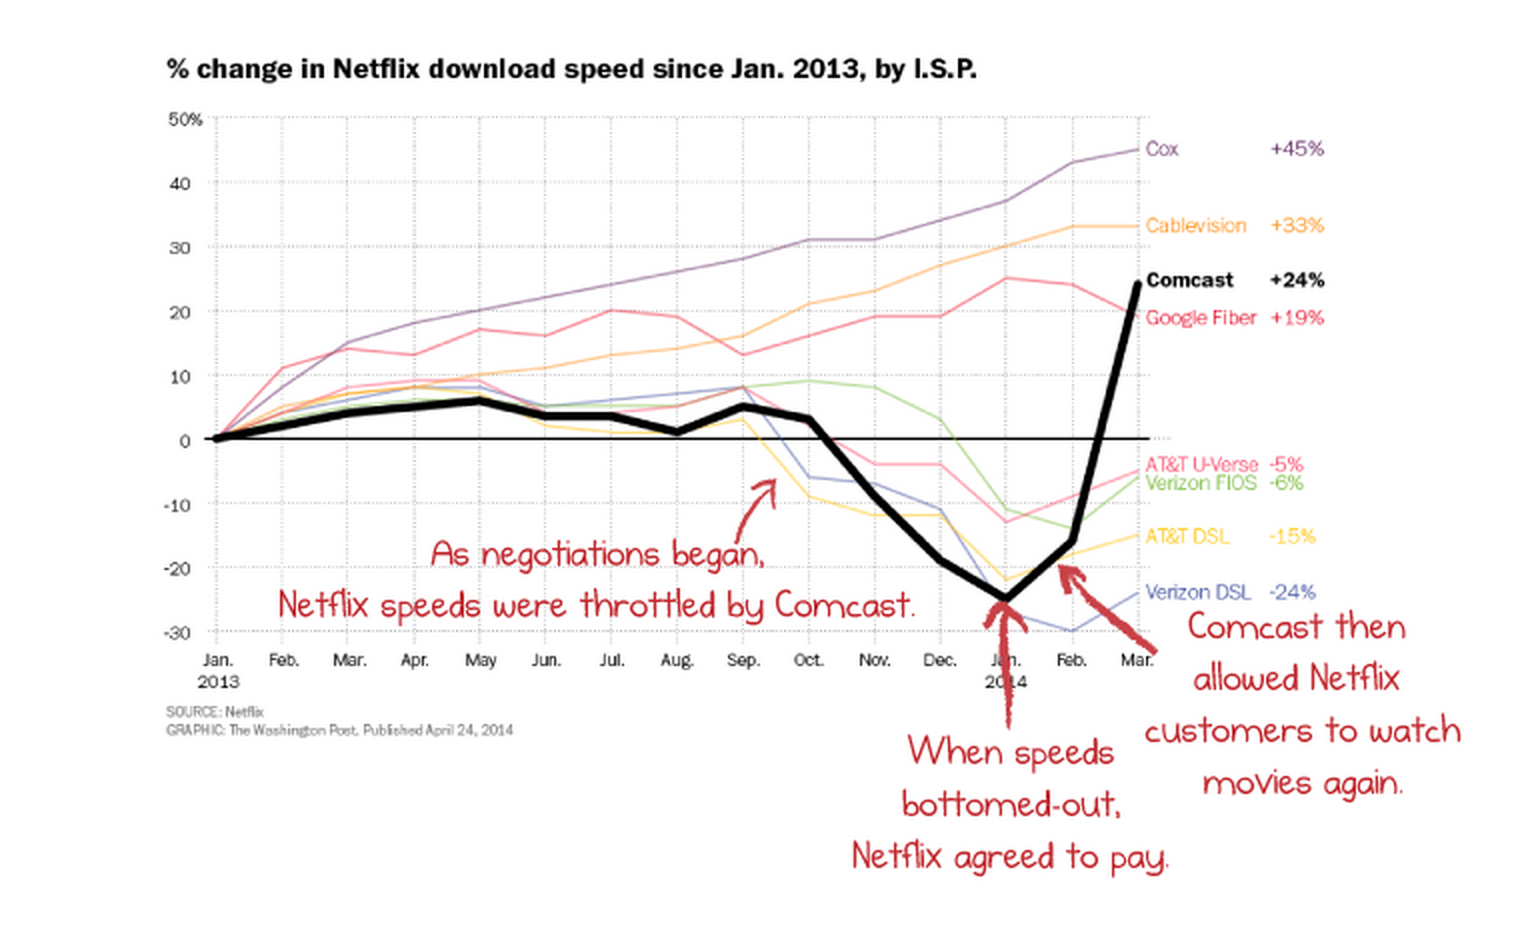
\includegraphics[scale=.20]{NetflixGraph.png}


\hspace*{-0.6cm}
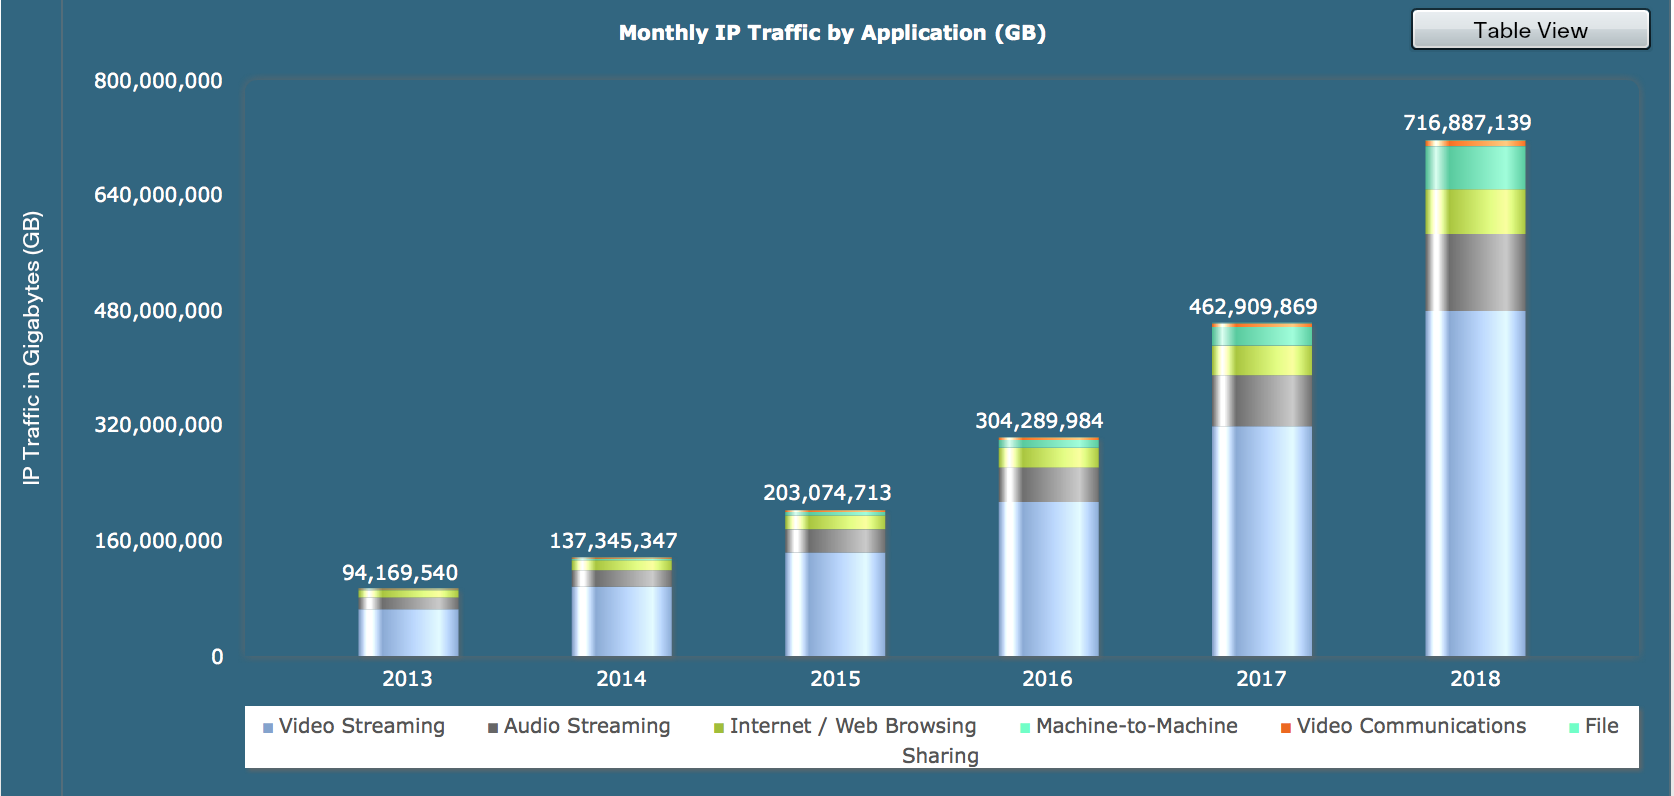
\includegraphics[scale=.29]{BandwidthGraph.png}


\subsection{Net Neutrality in Europe}

In April of 2014 the European Union (EU) passed telecoms law reform that defined and protected Net Neutrality [https://gigaom.com/2014/04/03/european-parliament-passes-strong-net-neutrality-law-along-with-major-roaming-reforms/]. This reforms happen close after the Netflix deal with Comcast and Verizon were approved in United States. In particular, amendment 235 gives a strong definition of “specialized services”, and amendment 236 specifies that this specialized services shall only be provided if the network capacity is sufficient. The fact that amendment 235 gives a strong definition of “specialided services” 


\subsection{Economic and Business Implications}
A major concern of te
Innovation
Feasibility
Economic/Infrastructure
Network efficiency



\section{Conclusions}
We have concluded that ISP....



\bibliographystyle{unsrt}
\bibliography{bib}

\end{document}
